% Created 2021-01-08 Fri 09:56
% Intended LaTeX compiler: pdflatex
\documentclass[11pt]{article}
\usepackage[utf8]{inputenc}
\usepackage[T1]{fontenc}
\usepackage{graphicx}
\usepackage{grffile}
\usepackage{longtable}
\usepackage{wrapfig}
\usepackage{rotating}
\usepackage[normalem]{ulem}
\usepackage{amsmath}
\usepackage{textcomp}
\usepackage{amssymb}
\usepackage{capt-of}
\usepackage{hyperref}
\date{\today}
\title{}
\hypersetup{
 pdfauthor={},
 pdftitle={},
 pdfkeywords={},
 pdfsubject={},
 pdfcreator={Emacs 27.1 (Org mode 9.3)}, 
 pdflang={English}}
\begin{document}

\tableofcontents

\textbf{Introduction to the subject of electronic music}

\section{Overview}
\label{sec:orgbbc2ba6}
\subsection{Course Structure}
\label{sec:org54ab31b}
The lectures are designed as an introduction to Electronic Music,
Sound Design and Creative Programming. There are 10 dates for lectures
that  allow us to make this brief introduction. Us refers to the
teachers,  students and me the course lecturer as well as the author
of these notes.  Throughout the course, an informal and personal way
of addressing  will be used to explain specific tasks and convey
information.  This will be familiar to those who have attended
lectures at the  Vienna Music Institute as well as something new to
some  who are used to the more formal approach.

One of the key principles we will focus on over the next semester is
the  idea of ​​parametric design. And, in essence, this series of
lectures  can be described in detail as a general introduction to some
basic principles of parametric design. At lecture 5, this topic will
be  presented in detail, it will be enough for us now and in the
upcoming  lectures to get to know the individual modules such as
oscillators,  filters, amplifiers, sequencers and aspects of control. 


\subsection{Teaching Philosophy}
\label{sec:org7b86164}
The subject can be subdivided into the following categories

\begin{itemize}
\item Project Organisation
\item Sound Design
\item Sound Synthesis
\item Digital Signal Processing (DSP)
\item Function and algorithm design
\item Parametric Control
\end{itemize}

In creating these categories, I’ve tried to represent some of the core
principles of electronic music and also to do this in a way that
allows  some access to the first principles at the root of design and composition. 

\subsection{A Symbolic Patch Language for Electronic Music}
\label{sec:org96cfd8e}

To represent particular concepts, we‘ll be using a graphical patch
language  throughout the course. It will help to know for now some of
the basic elements, objects or modules that we will need to
represent. 

\begin{verbatim}

[osc]        <amp>        |\env/|        *filt*        °°seq°°        

dac|>        |<adc

\end{verbatim}


It might help to think about a patch as a kind of instrument, and these modules as the individual parts of that instrument. Surprisingly, it‘s not always immediately obvious to everyone that a guitar is created by setting together a number of parts like: strings, body, neck, fret board, bridge, etc. The manner of construction has been informed by the physical principles of acoustics and also the practical necessities of musicians. In this course it will be of huge advantage to you to understand some basic things about acoustics and your own practical needs as a musician. Of course, we won‘t be making guitars, but as I already mentioned, it helps to think about creating electronic music in terms of putting together instruments and using them to create music. 

\subsection{Portability}
\label{sec:orgc19057a}
The aim of the lectures is to learn the basics of electronic music. In this sense, we focus primarily on the principles and techniques that apply to the creation of electronic music, and secondarily on the learning of paradigm-specific methods.
In any case, basic principles can best be illustrated by practical examples. Sometimes it's easier for me to introduce certain concepts in the classroom with proprietary software. In such cases, the goal should not be to spend all your money on acquiring copies of the software you are using, but to find out how the techniques described can be practiced with freely available software. In the first place, you should use two programs in combination to work through the examples that appear in each lesson and work as homework assignments: VCV Rack and Reaper. 

\subsection{Reading Material}
\label{sec:org0bc13e1}

A very good resource if you want to brush up on some of the basics of the types of mathematics that are found at the root of musical systems
\begin{itemize}
\item Gareth Loy, \textbf{Musimathics vol. I-II}, MIT Press
\end{itemize}

Great reference for many of the essential topics of computer music
\begin{itemize}
\item Curtis Roads: \textbf{The Computer Music Tutorial}, MIT Press
\end{itemize}

Very well written book on modular synthesis, with lots of worthwhile exercises that will form the basis of our practical work throughout the course
\begin{itemize}
\item Allan Strange: \textbf{Electronic Music Systems Techniques and Controls}, Wm-C Brown Company Publishers, 1972
\end{itemize}


\section{Some fundamentals of Audio Synthesis}
\label{sec:orge00553d}
\subsection{Oscillators and Wave-forms}
\label{sec:org484e0a8}
Typically an oscillator will be at the root of a synthesis patch. 
In order to hear a specific pitch, one can set the oscillator to 
generate a voltage at the desired frequency.  
Note that there is also a relationship between pitch and perceived 
loudness: a tone played at 1024Hz will sound louder than a tone played with the same gain at 64 Hz.

\subsubsection{Sine Waves and the Harmonic Series}
\label{sec:orgffbc3b8}
Come to think of it, this could be a good time to mention the harmonic
series, we'll come back to the relationship between pitch and loudness
in a minute. 

\begin{center}
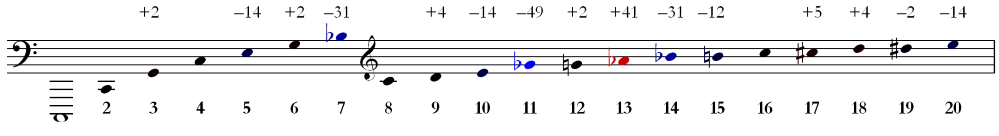
\includegraphics[width=.9\linewidth]{./images/Harmonic_Series1.png}
\end{center}

In the world of synthesizers and especially electronic music, an
oscillator will typically be looking for a precise definition of pitch
in order to produce a tone. 

\begin{center}
\begin{tabular}{lrr}
Pitch name & partial num. & Frequency (Hz)\\
\hline
c, & 1 & 64\\
c & 2 & 128\\
g & 3 & 192\\
c' & 4 & 256\\
e' & 5 & 320\\
g' & 6 & 384\\
bf' & 7 & 448\\
c'' & 8 & 512\\
d'' & 9 & 576\\
e'' & 10 & 640\\
gf'' & 11 & 704\\
g'' & 12 & 768\\
af'' & 13 & 832\\
bf'' & 14 & 896\\
b'' & 15 & 960\\
c''' & 16 & 1024\\
\end{tabular}
\end{center}


\begin{itemize}
\item base frequency = f\textsubscript{b}
\item partial number = p\textsubscript{num}
\end{itemize}

To calculate partial frequencies along the harmonic series:
\textbf{f\textsubscript{x} = f\textsubscript{b} * p\textsubscript{num}}

\begin{itemize}
\item eg: \textbf{f(11) = 11 * 64 = 704}
\end{itemize}

\subsection{A side note on midi to Hertz conversion}
\label{sec:orgd9c7ae2}
Practically speaking, you will rarely have to think about doing these
types of conversions from a specific pitch to a midi number. Midi is a
really useful protocol that maps an equal tempered tuning system to
integer values in the range of (0-127).

\section{Approaches to synthesis}
\label{sec:org1a54e41}

Here is a link to a very interesting website that depicts how the
basics of additive synthesis work. 

\url{https://teropa.info/harmonics-explorer/}

\subsection{Waveform Types}
\label{sec:org45d300a}
Of course, a spectrum analysis of the tone produced by a musical
instrument would reveal the presence of individual frequency
components. These are basically packets of energy focused around
certain points in time. Pythagoras or Plato or one of those fellows
would have probably started waxing lyrical about the harmony of the
spheres at this point. 
The main point here is that you don't need to think too deeply about
the concept of \emph{spectrum analysis} for now, maybe think about it as a
type of sonic x-ray that can reveal some interesting truths about the
nature of a sound. 
The whole point of mentioning analysis at all is that it can be quite
useful when used in combination with synthesis. If fact the practice
of the \emph{analytic-synthetic} method also goes all the way back to the
Greeks. But that's getting slightly off-topic.   

To summarize about wave-forms: depending on how they are combined,
simple sine-wave components can create more complex wave types. The
tones produced by musical instruments sound themselves complex and can
be analyzed to reveal the underlying structure. There are a few main
types of waveform that are typically found as settings on an oscillator.

\begin{center}
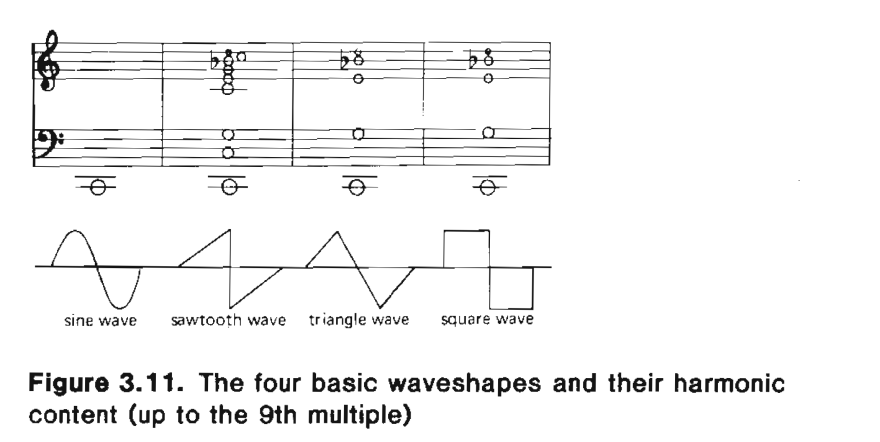
\includegraphics[width=.9\linewidth]{./images/waveforms.png}
\end{center}

\subsection{Oscillator Controls}
\label{sec:org03a1312}
\subsubsection{Tuning}
\label{sec:orgf5a5511}
\begin{itemize}
\item Offset
\item Fine-tune
\end{itemize}

Obviously, one of the first steps for most endeavours that involve
music, one of the first steps is to tune your instruments. Think about
a band or an orchestra that are going to play a specific melody
together, the instruments and voices need to all agree upon a specific
reference pitch and tuning system to play in before they start
thrashing out melodies and harmonies. 

This example of Ravel's Bolero is sometimes referred to as an example
of an "additive" musical structure. The way that he chooses to
orchestrate the melody is by calling for a number of different
instruments to "double" at different harmonic (as in series)
intervals. 

\#+ATTR\textsubscript{HTML} :width 50
\begin{center}
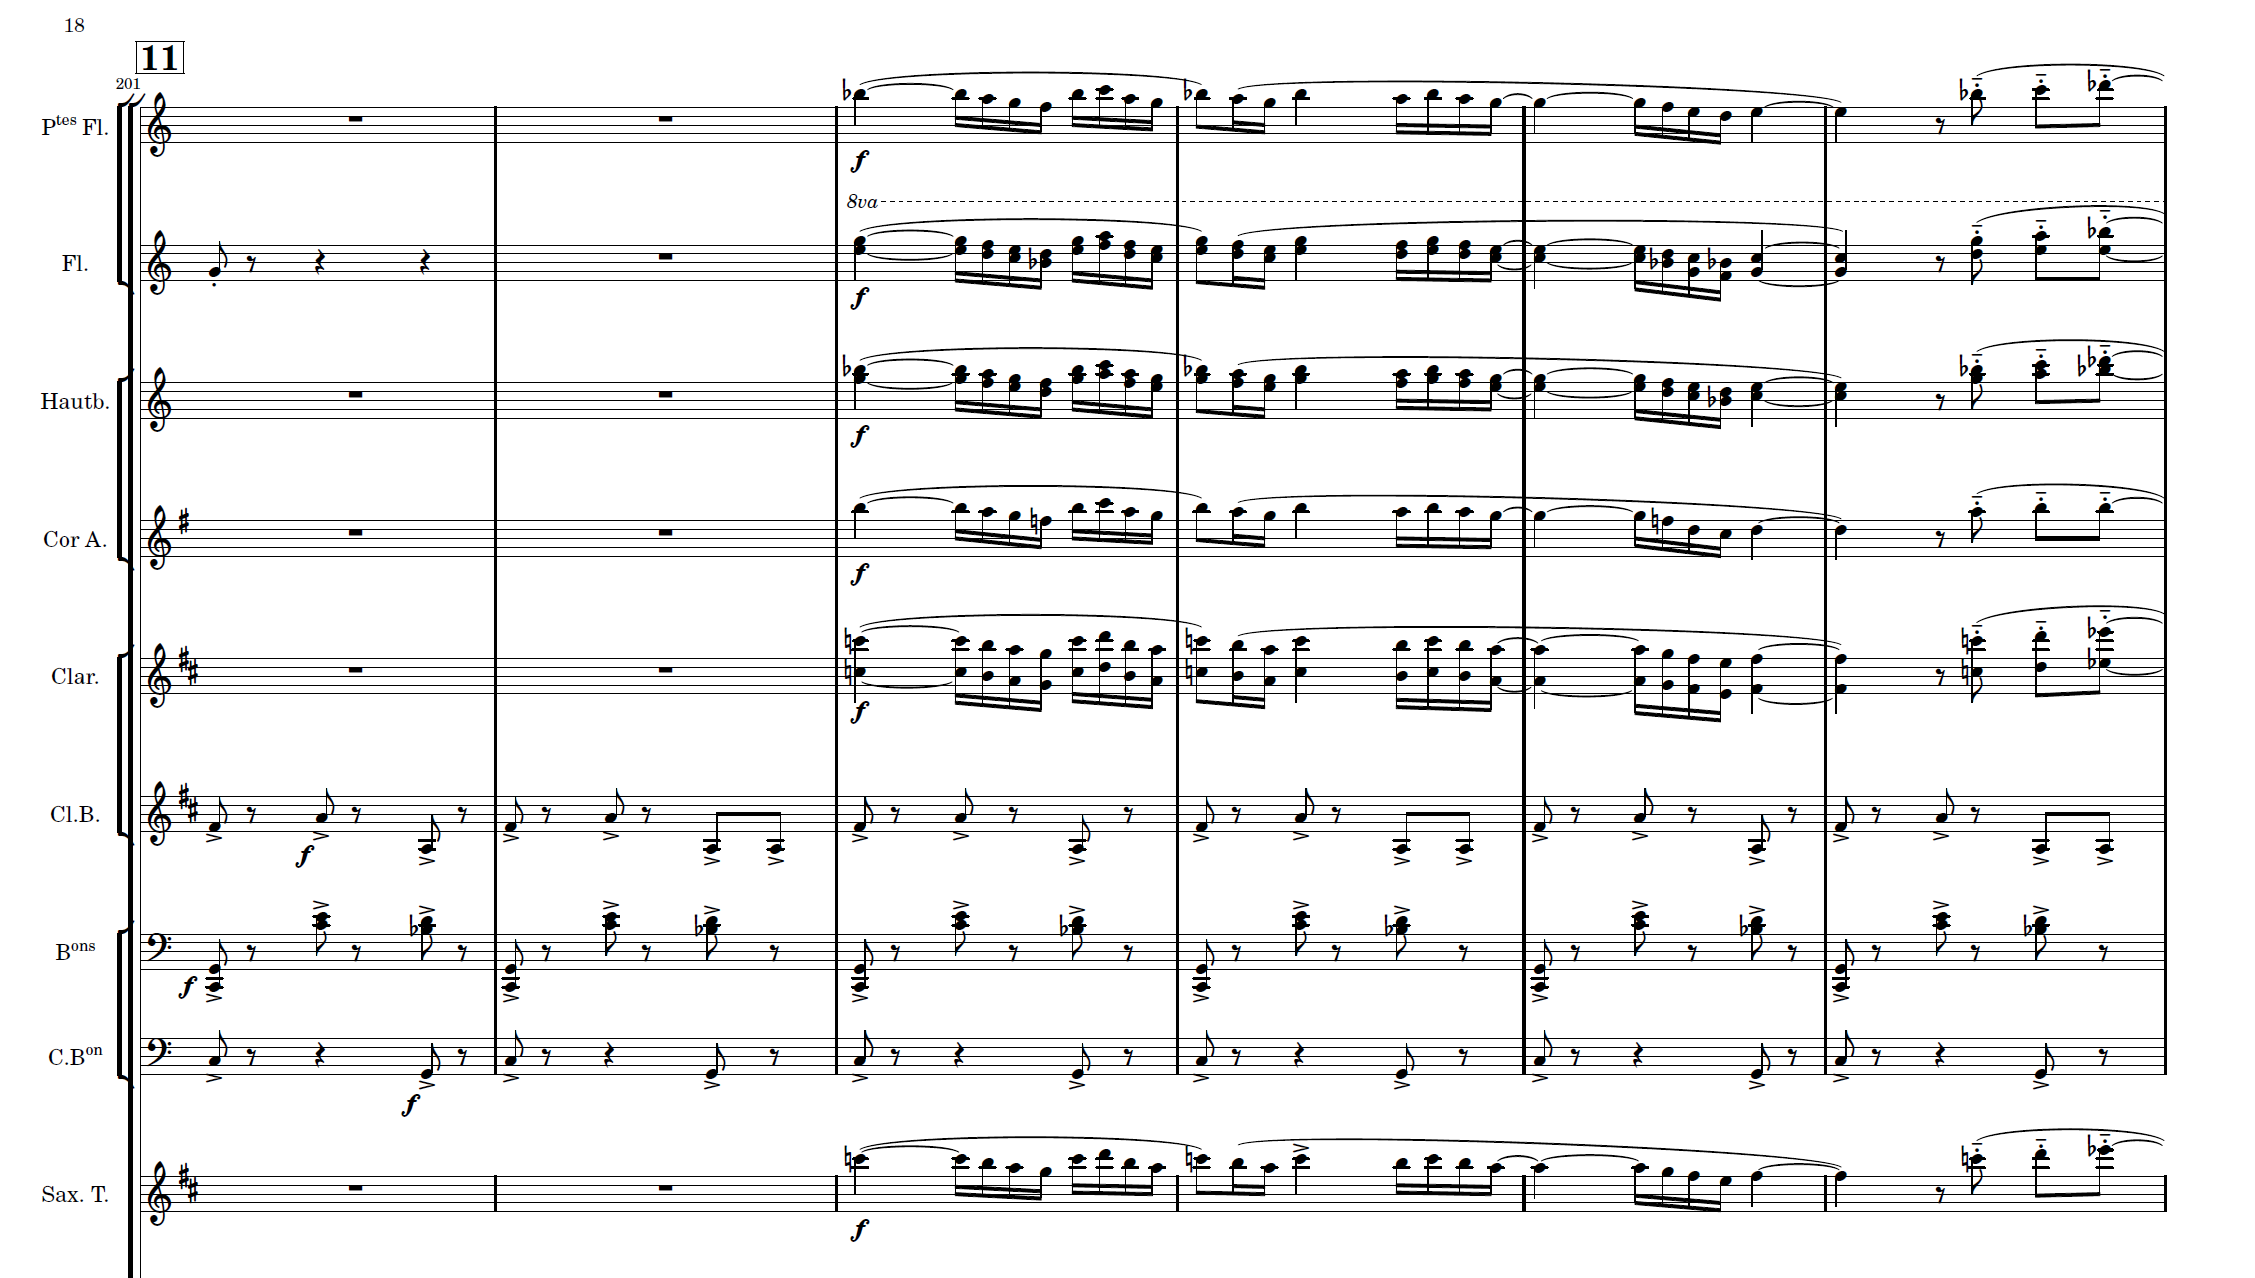
\includegraphics[width=.9\linewidth]{./images/ravel_bolero.png}
\end{center}


\subsubsection{Pitch input}
\label{sec:orgb10773e}
\begin{itemize}
\item Midi
\item Control Voltage
\end{itemize}

\subsubsection{Frequency Modulation (FM)}
\label{sec:org0585770}
We'll go into some more detail about frequency modulation (and
modulation in general) later on in the course. It just might be
useful to point out that most oscillators will typically have a
control for FM.

\subsubsection{Pulse width}
\label{sec:org559f3ce}
On the square wave setting, it is possible to control the length of
the \emph{duty cycle} of a square wave. Basically, if we were using the
oscillator to open some sort of a gate, the gate would remain open for
the length of time that the square wave is non-zero. 

\begin{verbatim}
      _____       _____       _____
     |     |     |     |     |     |
     |     |     |     |     |     |
_____|     |_____|     |_____|     |_____
      ___         ___         ___
     |   |       |   |       |   |
     |   |       |   |       |   |
_____|   |_______|   |_______|   |________
      _           _           _
     | |         | |         | |
     | |         | |         | |
_____| |_________| |_________| |__________

\end{verbatim}

\subsection{Additive Synthesis}
\label{sec:orga3be641}
Very simply put, additive synthesis is the idea of building up complex
sounds from very, very simply components. Most typically these are sin
tones. The link above connects to an interesting application written
in JavaScript. It's possible to see how the combination of different
sets of partials can produce specific wave shapes. 

\subsubsection{Building a Hammond organ}
\label{sec:org15af980}
This series of videos describes how to build a Hammond organ style
synthesizer using vcv rack: \url{https://youtu.be/kZJF50joo2w}


\subsection{Subtractive Synthesis}
\label{sec:orgd9ee3a3}

\begin{enumerate}
\item Envelopes
\label{sec:org30946e0}
In the patch below, we make reference to an "ADSR" envelope for the
first time. This refers to a transient generator that has four
components: Attack, Decay, Sustain and Release. Of these four, three
control temporal aspects of the transient waveform that is produced
(ADR) and the remaining control for sustain controls the amplitude of
the waveform after the decay from a peak amplitude is complete.
\end{enumerate}

\subsubsection{Basic Patch Structur}
\label{sec:org613f4bb}
\begin{center}
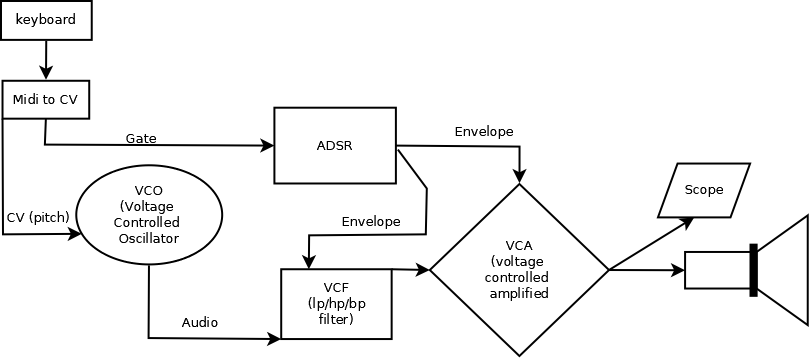
\includegraphics[width=.9\linewidth]{./basicSubtractive.png}
\end{center}

\section{Filtering techniques}
\label{sec:orgd55e2cb}
There are many interesting and musical ways to use filters in the
context of modular synthesis. This section briefly outlines some of
the initial approaches that might be interesting. It is highly
encouraged to do your own experiments with filters. Some basic initial
approaches are outlined below and demonstrated in the accompanying
patches. 

\subsection{Note on amplifiers and filters}
\label{sec:org6f47bcb}
It's worth pointing out at this point that there is a inverse proportianal
relationship between loudness and pitch. Basically, as the pitch
increases, a decrease in gain is necessary in order to maintain the
same dynamic. The opposite is also true, when lowering the pitch, it
is important to increase the gain in order to maintain the same
dynamic level. 

Another thing that's worth mentioning is that it's useful to think of
a filter as basically a very specific type of amplifier i.e. one that
selectively amplifies components of a signal depending on the settings
that are "programmed" in by the user / sound designer or audio
developer. The specific "type" of filter (LP/HP/BP\ldots{}) determines to a
large degree what specific functionality is available. 

\subsection{Low Pass Filters}
\label{sec:org1598f14}
Everything above the \textbf{cutoff} frequency is filtered out. For most
musical uses, the filter cutoff will be controlled 

\subsubsection{Control of Cutoff via Envelope}
\label{sec:org35825ba}
This is the case that we documented in the patch \emph{classicSutractive}
where a single ADSR envelope is used to control the amplitude and
frequency of the sound. 

\subsubsection{Control of Cutoff via Offset and Track}
\label{sec:orga074acb}
In this case, the filter cutoff is tuned to a particular offset
value (e.g. 8ve + 5th above root) this ensures that the resultant
sound has a stable spectrum because it always contains the same
frequency components. 

In the example \emph{trackingSubtractive} the VCO is tuned to  261.63 Hz
while the cutoff of the filter is offset to a value 1.5 times higher
than this (261.63 * 1.5 = 392.445)

In the patch \emph{lp\textsubscript{integralNoise}} two banks of filters are used. They are
tuned to a natural harmonic seventh chord (1, 2, 5, 7) partials. The
resonance on the first bank is turned up to full so that the filters
go into self oscillation. The second bank receives audio input from a
white noise source, in order to "fill out" any partials that lie below
the control signal that is used to change the cutoff frequency.

\subsection{High Pass Filters}
\label{sec:org28896f6}
As you might expect, high pass filters pass all frequencies that exist
above a certain cutoff. When applied to a single waveform coming from
an oscillator source, the sound is the quite familiar sweep up the
overtone series. 

However, when used on multiple simultaneous waveforms, hp filters can
be a useful way to create new and interesting tone colors that would
otherwise be difficult to achieve. 

The patch \emph{hp\textsubscript{colorExploration}} contains two oscillators that are
producing triangle waves tuned to a perfect major third in a low
register. When we apply a high-pass filter to eliminate the lower
harmonics, we are left with some uncanny tonal textures. The filter
cutoff can be changed either manually or automated by using the output
of a low frequency oscillator (LFO).  

\subsection{Band Pass Filters}
\label{sec:orgbb6689f}
Another commonly occuring type of filter is the band pass filter, this
is basically a combination of lp and hp, so everything but a narrow
"band" of frequencies in the middle of the spectrum is filtered
out. There are some really interesting ways to use this technique. 

The patch \emph{bp\textsubscript{colorExploration}} iterates on the previous patch, the
oscialltors are tuned to a more "stable" perfect fifth and the output
of the high pass routed into a second low pass filter. This means that
many of the high end noise that was occurring in the previous examples
can be filtered out and for a more predictable "harmonic" result.





\section{Musical Signals}
\label{sec:orge12e175}
\subsection{Simple Control of Pitch using LFOs}
\label{sec:orgd3fdafc}
LFO = low frequency oscillator

Range of audible frequencies 15 - 20.000Hz -> stuff that can be heard
as a pitch!

That means anything below 15Hz doesn't sound

\subsubsection{The value of Hertz}
\label{sec:org7c0dab0}

1 Hertz = 1 cycle of a waveform per second
1 cycle per second = 60 cycles per minute
Tempo of a 1 Hz LFO = 60 BPM clock

\subsubsection{Pitch sweep}
\label{sec:org63cc852}
This possibly the most simple type of functionality and can be achieved
pretty easily. Simply connect the output of an LFO to the pitch input
of an oscillator that is tuned to sound at audio rate. There are a few
things to note:
\begin{itemize}
\item If you want to have control over the range of pitch that gets
sweeped, you need to include an attenuator in the signal path
\item The pitches output are unquantized (they don't conform to any
particular scale)
\end{itemize}

\subsubsection{Sample \& Hold}
\label{sec:orgc343646}
The first step towards getting the sort of discrete steps that we
would need to make up a musical scale is isolating individual pitches
within the context of our filter sweep, and ensuring that the control
signal ("CV") stays at one specific pitch long enough for us to
perceive it as a note. See the patch "sampleHold1.vcv" for details on
how to patch this up.
In this patch we are introducing the "Random" module, an interesting
base module in the VCV suite. It is programmed to generate random
values along one of two possible distriubutions. These random voltages
are sampled according to the rate function, and they can be further
divided up into a maximum of 16 steps using the "shape" slider. It's a
useful module and I highly recommend reading the short documentation
to get a better understanding of what it does. 

Some notable features of this pitch. 
\begin{itemize}
\item At this stage, we might seem to be approaching something that could
possibly be described as a musical signal.
\item With some clever routing of our modules, we can also control other
aspects of the sound
\end{itemize}


\subsection{Sequencers}
\label{sec:org806b47c}
\subsubsection{Modular Style}
\label{sec:orgf84e064}
The most typical style of sequencer found in modular systems are those
with rows of pots (basically potentiometers) that are used to regulte
the outgoing cv. There is either an internal clock that powers the
steps, or the sequencer is fed in a clock pulse from an external
source. 
A pot is used to set the specific voltage at a given step, and then
this gets combined with a gate signal that is typically used to
trigger some sort of an envelope. This means that the modular style
sequencer's output is usually routed to two sources. 

\subsubsection{DAW Style}
\label{sec:orgeda4b4a}
The "piano roll" is one of the most common ways to sequence in a daw,
basically this is a graphic user interface that maps an image of a
piano keyboard on to the screen and the user basically drops in notes
where they would like them to sound. Sequences can typically be of
variable length.


\subsection{Quantization}
\label{sec:orga130760}
\subsubsection{Pitch Quantization}
\label{sec:orgdca9506}

Oscillators are outputting an audio signal, the pitch control is
enabling control over what frequencies are being put out. For all
intents and purposes this control enables continuous access to all
pitches along the frequency spectrum. If we don't impose any rounding
on these values as they come out of the oscillator, we refer to the
audio signal as unquantized. 

Although obviously it can be applied to pitch very effectively,
quantization steps can be applied to "CV" signals also. This means
that you can basically run a control signal through a quantizer in
order to "whip it into shape" before passing it to the CV input of an
oscillator. 

\subsubsection{Offsets \& Harmonization}
\label{sec:org6c9469d}
While we're on the topic of quantization, another cool thing that you
can do with quantizers is to use them in combination with some
offsets. 
Basically, you can take a single cv signal and pass it through an
offset/attenuator in order to change the range and amplitude of the
signal. If you pass the offset signal back into a quantizer tuned to
the same pitches as your second signal, you get instant access to
diatonic or tonal harmonization. 

One further interesting thing to try out is to further mix the offset
signal with another signal coming from an LFO. This quickly gives rise
to many variations on the original seuqence, as it is harder to
predict exactly how the sequences are related to one another.

\subsubsection{Clock Subdivision}
\label{sec:org972eaa9}
In order to have a bit more control over what's coming out of the
quantizer, it's often useful to use a clock multiplier/divider to
create a rhythmical relation to the amplitude envelope of your second
signal. 


\section{Troubleshooting}
\label{sec:orgb25c3dc}

\subsection{Patch description}
\label{sec:orgfdb1449}

\begin{itemize}
\item We're sending noise to a filter
\item Want to control the filtercutoff with a keyboard
\item We want a pitched noise output
\end{itemize}

\section{Modulation}
\label{sec:orgfd8fb63}
\subsection{Sub-Audio Rate Modulation}
\label{sec:org5093aac}
\subsubsection{Definition}
\label{sec:org7877afb}
When we're taking about modulation, typically we differentiate between
two different types of signal that are involved:

\begin{itemize}
\item the \textbf{carrier} is basically considered the basis for the modulation,
the tone that gets manipulated or that "carries" the modulator
\item the \textbf{program or modulator} is the signal that is causing some sort of
periodic fluctuations to the carrier
\end{itemize}

If you're using a Low Frequence Oscillator to some how "animate" the
signal on it's way to becoming audio, you can pretty much consider
this sub-audio rate modulation. As we've mentioned before, anything
that occurs below 15hz is below the threshhold for what humans can
perceive as pitch and so instead we typically here it as rhythm. 

\subsubsection{Amplitude Modulation (AM)}
\label{sec:org1e9513f}
If we're using an lfo to do amplitude modulation, then we are
typically mixing together the signal coming from an LFO with the
transient that is creating our envelope. This produces a kind of
"amplitude vibrato" where the volume of the tone seems to flutter. 

\subsubsection{Frequency Modulation (FM)}
\label{sec:orgb0d9c3e}
If the carrier is applied to the FM input of the modulator, then the
audible effects resemble that of a tremolo between two distinct
pitches.

\subsection{Audio Rate Modulation}
\label{sec:org74b2e6e}
\subsubsection{Side bands and Timbre}
\label{sec:orgb9f522e}
\subsubsection{FM}
\label{sec:org2f92110}
\subsubsection{AM}
\label{sec:org1240494}



\section{Sound Synthesis}
\label{sec:orgb5c6a6f}

The following is a cherry-pick and very brief exposition of a couple
of topics related to an area of sound synthesis that I've found
personally interesting over the years. These topics are all covered in
excellent detail in Gareth Loy's book Musimathics vol. II. 

\subsection{Delay Lines}
\label{sec:org9acf961}
Following on from the books disucssion, here are two ways to implement
a delay line. Although we haven't been worrying about the details of
implementation throughout this course, it's not a bad idea to
occasionally point to one or two as if we are serious scholars. As an
aside, I once submitted PhD application to Trinity College Dublin with
the glorious notion of writing my dissertation on "something about
time". If nothing else, this brief discussion of exactly what a delay
is might serve as a reminder that all of this music stuff seems to
have something or other to do with time.

\subsubsection{Mexican Wave}
\label{sec:org7b9755e}
(The actual example in the book is Bucket Brigate, but I've always
been a big personal fan of the mexican wave). Imagine that the year is
\begin{enumerate}
\item The FIFA world cup is on and you have tickets to the final where
\end{enumerate}
Argentina play against West Germany. At different points during the
match, the crown begins "passing a wave" around the stadium. The idea
is that the peak of the wave is passed by one section of the crowd
standing up and then returning to their seats as the peak moves to the
next acjacent section.
\url{https://en.wikipedia.org/wiki/File:AUSvIRE4Wave.ogv}

For the Bucket Brigade or Mexican Wave analogy to work, you have to
put yourself in the position of imagining that you are the peak of the
wave travelling around the stadium, you are essentially being passed
from one section of the crowd to the next.

To bring the anology a bit closer to the computer, imagine the
sections of the crowd as an array of samples, each time the "wave"
passes along the array, a sample is moved from one index to the next,
or from the input stack to the output stack along a FIFO (first in
first out) queue. This is not to be confused with FIFA of course,
which stands for the Fédération Internationale de Football Association.

\subsubsection{In-place method}
\label{sec:org96ccd20}
The inplace method is the same as above, there is a queue and an input
and output stack, but this time for the analogy you have to imagine
yourself as an individual in the crowd. You experience the peak of the
wave when it passes, and then you have to sit and wait again for n
seconds for the wave to come around a second time.

\subsubsection{Echo modelling}
\label{sec:org821942d}
Imagine a signal path: 
\begin{verbatim}

(sound source) -> [ADC] -> [---delay---] -> [DAC] -> |) 

\end{verbatim}

If you place a delay module in the signal path and that delays the 
sound by \emph{N} samples. The sound will arrive at the output \emph{N} seconds
after the sound has left the input.

\subsubsection{Screaming into a cave}
\label{sec:org0f4f176}
At one time or another, we've all screamed into a cave. Not the empty
cave of our dreams, but a real physical cave with damp, stalactites
and formerly bears. You may recall that the echo that you hear
dissipates on it's return. Well, this dissipation is something that we
can try to model with our syntehsis system in order to recreate an
accurate sounding audible delay. 

In real world acoustical situations (i.e. a room full of air) the
pressure of a transverse, spherical waveform drops off at 1/d. That is
to say the amplitude decreases as the delay time increases. 

If the delay line is \emph{N} samples and \emph{T} seconds long, it's possible
to model the attenuation of a pressure wave by setting a = 1/(\emph{NT})
Intesity (perceived loudness) drops off as d\textsuperscript{2}, so we can write 
a = 1/(\emph{NT})\textsuperscript{2}

\subsubsection{Mercilessly skipping ahead to some sound examples}
\label{sec:orgffe7e41}

Okay, so real physical situations are a bit more complicated that this
simple model. Typically if there is a sound source playing in a room,
the room will give back many more reflections than the sound
source. This is also true for the bodies of instruments, where tiny
reflections can give a specific violin, cello, guitar, drum, marimba,
its own very distinctive quality. There is a whole area of synthesis
research known as physical modelling, where the various types of delay
networks are compiled to create many interesting sounds. 

\subsection{Karplus strong}
\label{sec:org7dccc04}
Physical modelling synthesis sort of begins though in a very simple
way, with a type of algorithm known as karplus strong. It's very
simple infact, all you need is a noise source, an amplifier, a vca and
an output. By modulating aspects of the delay time and feedback, you
can recreate the sound of a pitched string.

I've created a patch called "karplus-really-Strong.vcv" to demonstrate
some of the tecniques mentioned above.

\section{Project work}
\label{sec:org13af9a6}
\subsection{in a DAW}
\label{sec:org544126a}
\subsection{Voice Assignment}
\label{sec:orgd828315}

\subsection{Appendix A}
\label{sec:org931e284}
\subsubsection{Program selection, installation and directory structure}
\label{sec:org18791f1}
\subsubsection{Project organisation in Digital Audio Workstations}
\label{sec:orgfc0af38}
\end{document}
